\documentclass[10pt]{article} 
\usepackage{ctex}
\usepackage{graphicx}
\usepackage{amsmath}
\usepackage{epstopdf}
\usepackage{tabularx}
\usepackage{geometry}
\usepackage{float}
\usepackage{listings}
\usepackage{xcolor}
\usepackage{fontspec}
\usepackage{color}
\geometry{right=1cm,left=1cm,top=1cm,bottom=1.5cm}
\definecolor{vgreen}{RGB}{104,180,104}
\definecolor{vblue}{RGB}{49,49,255}
\definecolor{vorange}{RGB}{255,143,102}
\lstdefinestyle{verilog-style}
{
    language=Verilog,
    basicstyle=\small\ttfamily,
    keywordstyle=\color{vblue},
    identifierstyle=\color{vblue},
    commentstyle=\color{vgreen},
    numbers=left,
    numberstyle=\tiny\color{black},
    numbersep=10pt,
    tabsize=8,
    moredelim=*[s][\colorIndex]{[}{]},
    literate=*{:}{:}1
}
\makeatletter
\newcommand*\@lbracket{[}
\newcommand*\@rbracket{]}
\newcommand*\@colon{:}
\newcommand*\colorIndex{%
    \edef\@temp{\the\lst@token}%
    \ifx\@temp\@lbracket \color{black}%
    \else\ifx\@temp\@rbracket \color{black}%
    \else\ifx\@temp\@colon \color{black}%
    \else \color{vorange}%
    \fi\fi\fi
}
\makeatother
\usepackage{trace}
\title{流水线设计大作业}
\author{王炜致\ 2022010542}
\date{}
\begin{document}
\maketitle 
\section{实验目的}
通过将单周期处理器改造为流水线处理器的实践操作,
深刻领会并巩固《数字逻辑与处理器基础》课程中
所学处理器相关知识,
重点掌握汇编指令、冒险处理、外设等的架构与设计,
提高汇编语言及verilog硬件描述语言的理解与编程能力,
体会处理器的设计及优化升级过程。
\section{设计方案}
\subsection{总体设计}
该流水线由《数字逻辑与处理器基础》课程中提供的单周期处理器
改造而来;此外,还沿用了理论课中编写的排序代码。
这两块基石的基本原理,在此不再赘述,以下展示的是利用
单周期处理器运行排序代码的结果,旨在证明单周期处理器代码
及排序代码(为适配处理器,略有修改)的可靠性。
\begin{figure}[H]
    \centering
    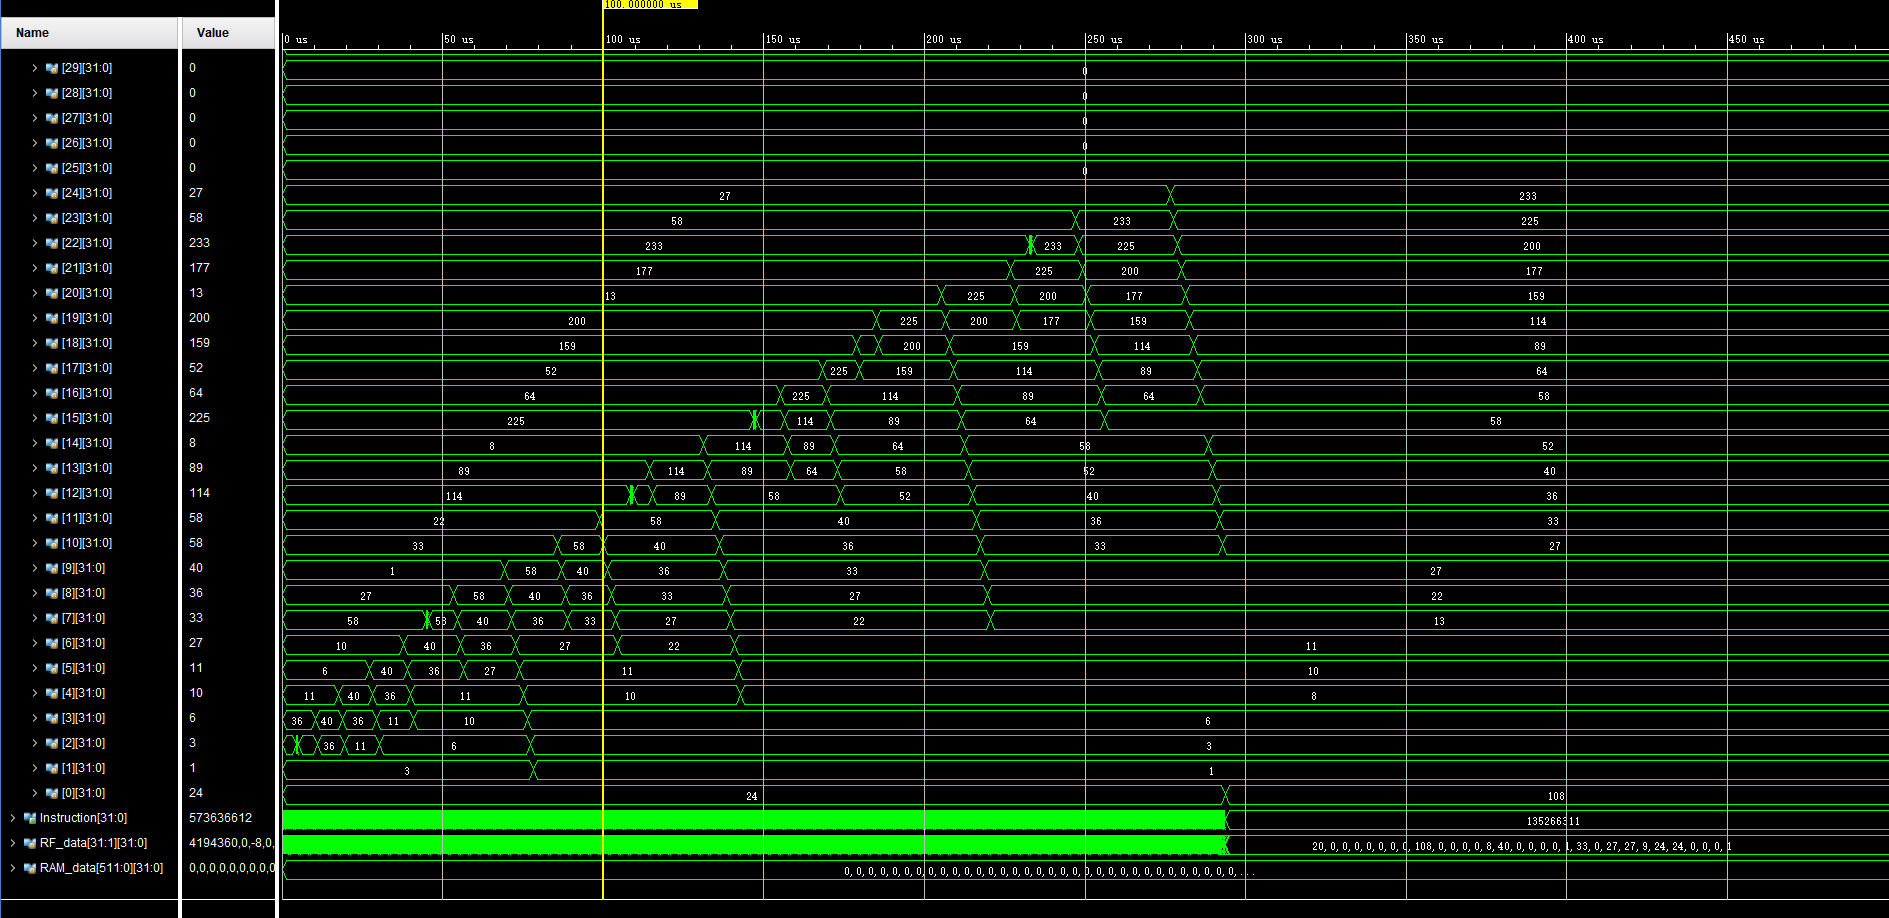
\includegraphics[scale=0.38]{MUCHOGUSTO.png}
    \end{figure}

在改造的过程中,

\subsection{指令集扩充设计}
根据指导书要求,参阅MIPS文档,扩充跳转与分支指令如下:
\begin{table}[h]
    \footnotesize
\begin{center}
    \begin{tabular}{|r|r|r|r|r|r|r|r|r|r|r|r|}
        \hline
        &PCSrc[1:0]& Branch & RegWrite & RegDst[1:0] & MemRead & MemWrite & MemtoReg[1:0] & ALUSrc2 & ALUSrc1 & ExtOp & LuOp\\
        \hline
        bne & 0(00) & 1 & 0 & x(xx) & x & 0 & x(xx) & 0 & 0 & 1 & x\\
        \hline
        blez& 0(00) & 1 & 0 & x(xx) & x & 0 & x(xx) & 0 & 0 & 1 & x\\
        \hline
        bgtz& 0(00) & 1 & 0 & x(xx) & x & 0 & x(xx) & 0 & 0 & 1 & x\\
        \hline
        bltz& 0(00) & 1 & 0 & x(xx) & x & 0 & x(xx) & 0 & 0 & 1 & x\\
        \hline
        jalr& 2(10) & x & 1 & 1(01) & x & 0 & 2(10) & x & x & x & x\\
        \hline
    \end{tabular}
\end{center}
\end{table}

相应地修改了控制信号生成模块Control.v及模块端口,详见所附源代码。

\subsection{测试数据设计}
设置数据内存大小为256个字。按要求,准备24个待排序正整数,
在DataMemory.v中初始化RAM_data[1:24],作为测试样例。RAM_data[0]
存储的是待排序正整数的数量。
\begin{lstlisting}[style={verilog-style}]
    parameter RAM_SIZE = 512;
    parameter RAM_SIZE_BIT = 8;
    reg [31:0] RAM_data [RAM_SIZE - 1: 0];
    ...
    if (reset) begin
            RAM_data[0] <= 32'h00000018; //numbers=24
            
            RAM_data[1] <= 32'h00000003; 
            RAM_data[2] <= 32'h00000028; 
            RAM_data[3] <= 32'h00000024; 
            RAM_data[4] <= 32'h0000020B; 
            RAM_data[5] <= 32'h00003406; 
            RAM_data[6] <= 32'h00000A0A; 
            RAM_data[7] <= 32'h0000F03A; 
            RAM_data[8] <= 32'h0000001B; 
            
            RAM_data[9] <= 32'h00000001; 
            RAM_data[10] <= 32'h00009021; 
            RAM_data[11] <= 32'h00000216; 
            RAM_data[12] <= 32'h00000072; 
            RAM_data[13] <= 32'h00000059; 
            RAM_data[14] <= 32'h00000007; 
            RAM_data[15] <= 32'h000003E1; 
            RAM_data[16] <= 32'h00000B40; 
            
            RAM_data[17] <= 32'h00000034; 
            RAM_data[18] <= 32'h0000009F; 
            RAM_data[19] <= 32'h000000C8;
            RAM_data[20] <= 32'h0000000D; 
            RAM_data[21] <= 32'h000000B1; 
            RAM_data[22] <= 32'h000000E9; 
            RAM_data[23] <= 32'h0000003a; 
            RAM_data[24] <= 32'h0000001B; 
        
            for (i = 25; i < RAM_SIZE; i = i + 1)
                RAM_data[i] <= 32'h00000000;
\end{lstlisting}
\subsection{MIPS指令设计}
MIPS指令主要分为两个部分:排序功能实现部分以及软件形式数显控制部分。

排序部分使用《数字逻辑与处理器基础》课程中设计的插入排序算法,详见所附源代码。排序
完成后,
\subsection{WELOG实验板行为设计}

\newpage
\section{流水线改造(无冒险处理)}
\begin{figure}[H]
    \centering
    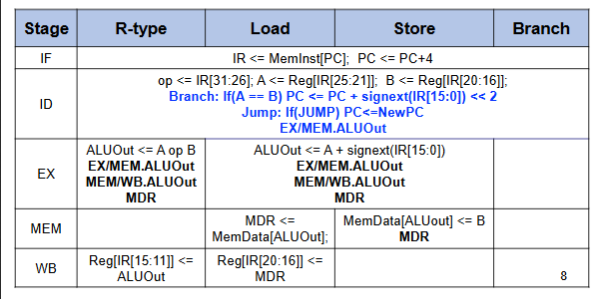
\includegraphics[scale=0.75]{table.png}
    \end{figure}
CPU.v的改动最大,需要在各模块输入/输出之间添加寄存器,以下
介绍寄存器的初步添加,不考虑冒险。

Control.v即控制信号模块在IF阶段调用,产生控制信号,为
传递控制信号,在CPU.v中插入IF/ID寄存器:
\begin{lstlisting}[style={verilog-style}]
	always @(posedge reset or posedge clk) begin//IF/ID PLUGIN BEGIN ↑IF
	   if (reset) begin
               IFID_Instruction <= 32'b0;
	       IFID_RegDst <= 2'b00;
	       IFID_PCSrc <= 2'b00;
	       IFID_Branch <= 3'b000;
	       IFID_MemRead <= 1'b0;
	       IFID_MemWrite <= 1'b0;
	       IFID_MemtoReg <= 2'b00;
	       IFID_ALUSrc1 <= 1'b0;
	       IFID_ALUSrc2 <= 1'b0;
	       IFID_ALUOp <= 4'b0000;
	       IFID_ExtOp <= 1'b0;
	       IFID_LuOp <= 1'b0;
	       IFID_RegWrite <= 1'b0;
	   end	   //more to consider
	   else begin
                IFID_Instruction <= Instruction;
	        IFID_RegDst <= RegDst;
                IFID_PCSrc <= PCSrc;
                IFID_Branch <= Branch;
                IFID_MemRead <= MemRead;
                IFID_MemWrite <= MemWrite;
                IFID_MemtoReg <= MemtoReg;
                IFID_ALUSrc1 <= ALUSrc1;
                IFID_ALUSrc2 <= ALUSrc2;
                IFID_ALUOp <= ALUOp;
                IFID_ExtOp <= ExtOp;
                IFID_LuOp <= LuOp;
                IFID_RegWrite <= RegWrite;
	   end
	end//IF/ID PLUGIN END ↓ID
\end{lstlisting}

ID阶段调用寄存器堆(读),注意WB阶段亦涉及调用寄存器堆(写),考虑
遵循先写后读原则(在RegisterFile.v中修改)。插入ID/EX寄存器:
\begin{lstlisting}[style={verilog-style}]

\end{lstlisting}

将Jump,Branch均置于ID阶段执行,则ALU不需要Zero。
无冒险处理的流水线例程测试如下:
\begin{figure}[H]
    \centering
    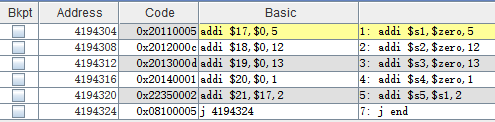
\includegraphics[scale=0.7]{hazardno.png}
\end{figure}
\begin{figure}[H]
    \centering
    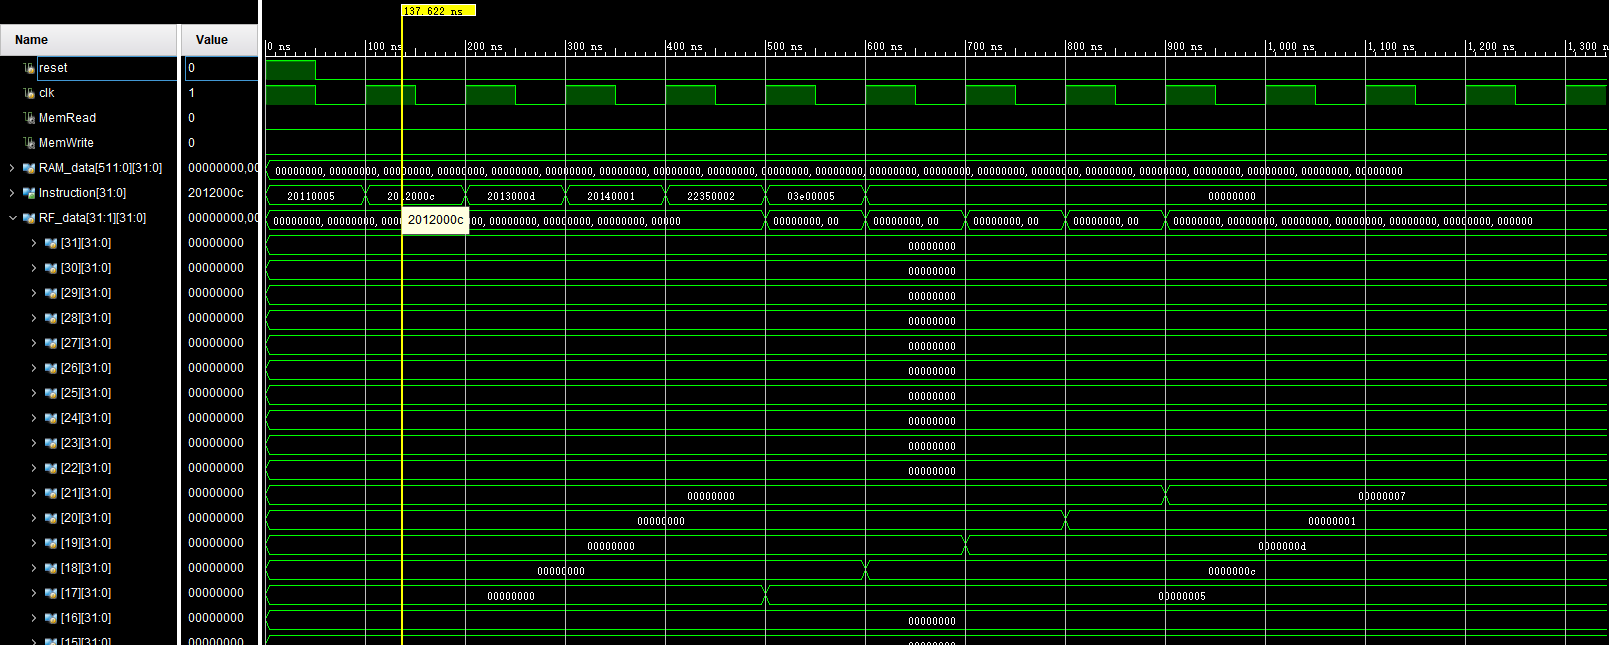
\includegraphics[scale=0.4]{norisk.png}
    \end{figure}
\newpage
\section{冒险处理}
\subsection{结构冒险}
InstructionMemory与DataMemory已作分离;R型指令
Mem阶段已空置;ALU已作功能疏解。
\subsection{数据冒险}
\subsubsection{同时读写寄存器堆}
\begin{figure}[H]
    \centering
    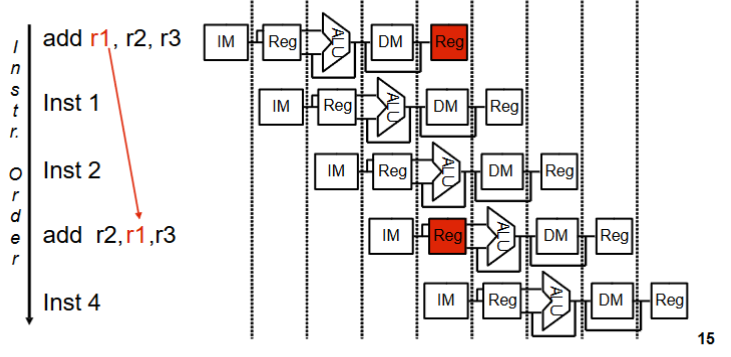
\includegraphics[scale=0.4]{reguse.png}
    \end{figure}

通过先写后读策略处理。利用always块的阻塞赋值实现代码执行的先后顺序。
\begin{lstlisting}[style={verilog-style}]
    always @(*) begin
        if (RegWrite && (Write_register != 5'b00000))
             RF_data[Write_register] = Write_data;//first write
        Read_data1 = (Read_register1 == 5'b00000)? 32'h00000000: RF_data[Read_register1];
        Read_data2 = (Read_register2 == 5'b00000)? 32'h00000000: RF_data[Read_register2];
    end
\end{lstlisting}
验证如下:
\begin{figure}[H]
    \centering
    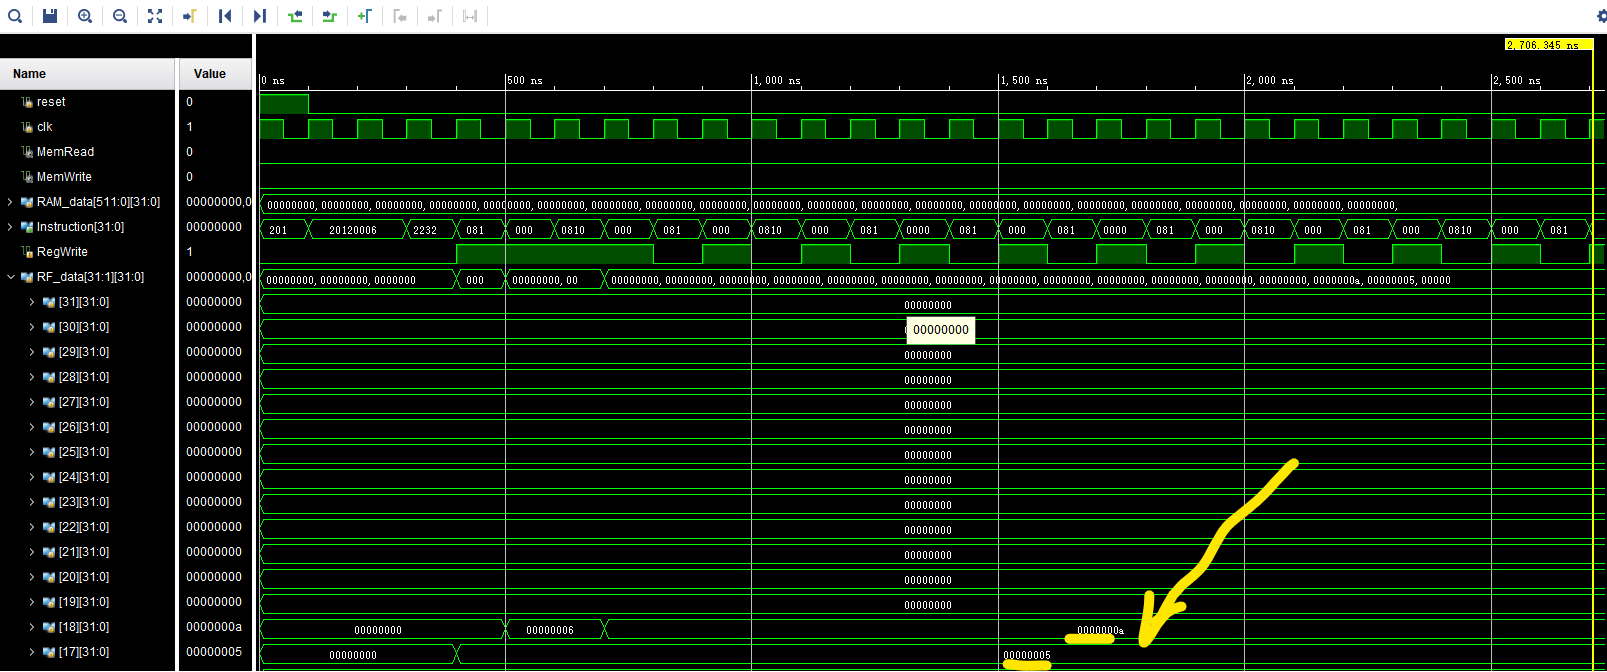
\includegraphics[scale=0.43]{fwtr.png}
    \end{figure}
    \begin{figure}[H]
        \centering
        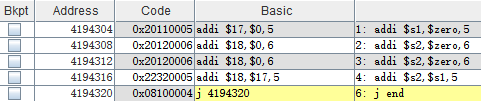
\includegraphics[scale=0.9]{fwtrx.png}
        \end{figure}
\subsubsection{时间顺序关联(ALU输出)}
\begin{figure}[H]
    \centering
    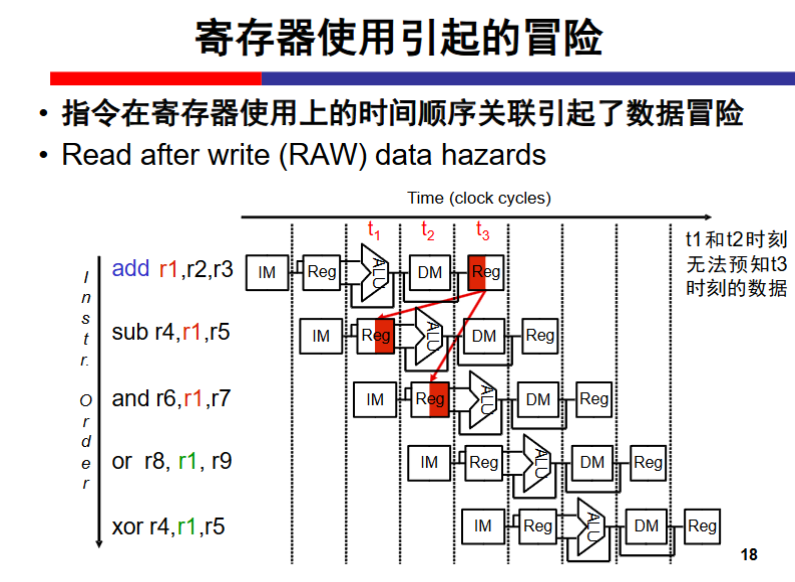
\includegraphics[scale=0.3]{reg.png}
    \end{figure}

ALU输出运算结果后,立刻转发给ALU输入端。需要修改ALU的输入端(二路),增加MUX选择合适的输入信号。
\begin{lstlisting}[style={verilog-style}]
    wire [32 -1:0] in1,in2;//rs,rt forwarding
    assign in1 = (~IDEX_ALUSrc1 && MEMWB_Memory_Read && MEMWB_Write_register 
        && MEMWB_Write_register == IDEX_Instruction[25:21])? MEMWB_MemBus_Read_Data:
        (~IDEX_ALUSrc1 && MEMWB_RegWrite && MEMWB_Write_register 
        && (MEMWB_Write_register == IDEX_Instruction[25:21])
        && (EXMEM_Write_register != IDEX_Instruction[25:21] 
        || ~EXMEM_RegWrite))? MEMWB_ALU_out:
        (~IDEX_ALUSrc1 && EXMEM_RegWrite && EXMEM_Write_register
        && (EXMEM_Write_register == IDEX_Instruction[25:21]))? EXMEM_ALU_out: 
        ALU_in1;
    assign in2 = (~IDEX_ALUSrc2 && MEMWB_Memory_Read && MEMWB_Write_register 
        && MEMWB_Write_register == IDEX_Instruction[20:16])? MEMWB_MemBus_Read_Data:
        (~IDEX_ALUSrc2 && MEMWB_RegWrite && MEMWB_Write_register 
        && (MEMWB_Write_register == IDEX_Instruction[20:16])
        && (EXMEM_Write_register != IDEX_Instruction[20:16] 
        || ~EXMEM_RegWrite))? MEMWB_ALU_out://mind load-store
        (~IDEX_ALUSrc2 && EXMEM_RegWrite && EXMEM_Write_register
        && (EXMEM_Write_register == IDEX_Instruction[20:16]))? EXMEM_ALU_out: 
        ALU_in2;
\end{lstlisting}
验证如下:
\begin{figure}[H]
    \centering
    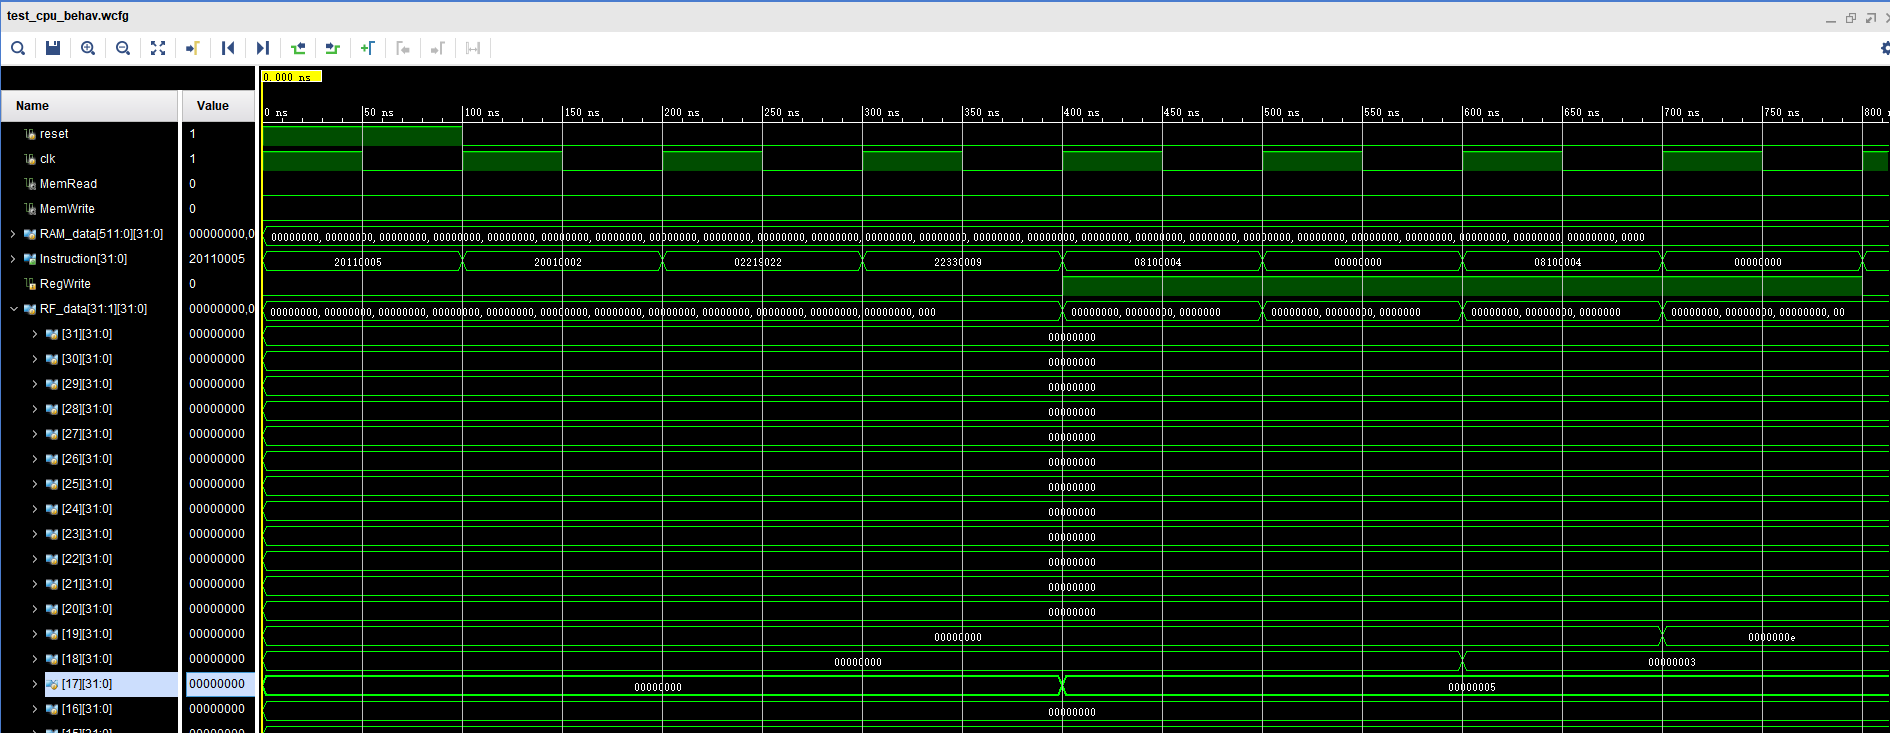
\includegraphics[scale=0.35]{haddaz.png}
    \end{figure}
    \begin{figure}[H]
        \centering
        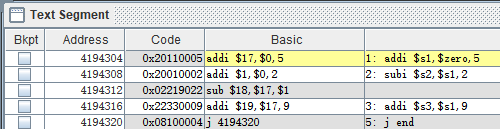
\includegraphics[scale=0.9]{hadd.png}
        \end{figure}
此外,若下一条指令为Branch(为简便,默认jr,jalr使用\$31,故不需要处理),
则不能不stall一个周期,再将数据转发到ID阶段。
验证如下:
\begin{figure}[H]
    \centering
    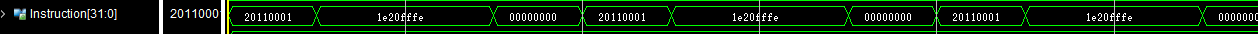
\includegraphics[scale=0.4]{bgtzz.png}
    \end{figure}
    \begin{figure}[H]
        \centering
        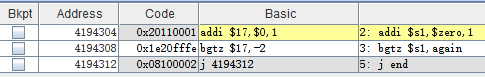
\includegraphics[scale=0.9]{bgtz.png}
        \end{figure}
\subsubsection{load-use冒险}
\begin{figure}[H]
    \centering
    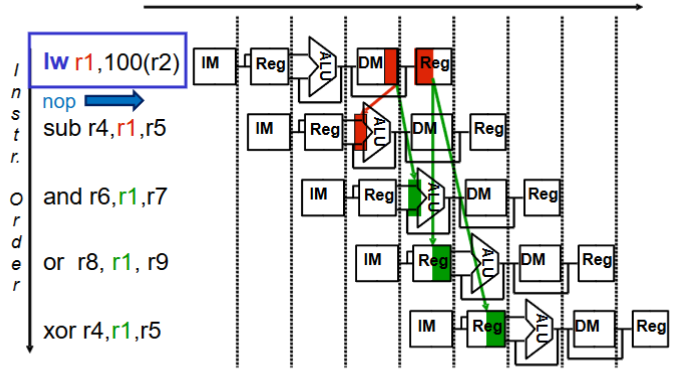
\includegraphics[scale=0.6]{load.png}
    \end{figure}
load-use冒险包含load-R类和load-store类冒险,前者不可避免地需要stall一个周期。
故需要将读出数据作转发。
处理load-store冒险时,在ALU输入forwarding条件中需要分辨立即数加法与寄存值加法;
DataMemory写端口也需要引入MUX作forwarding判断。

非常特殊的情况:
lw \$s1,4(\$zero),sw \$s1,0(\$s1),由于stall一个周期,无法由MEM/WB转发,同时\$s1尚未
更新。故需要特殊处理:
\begin{lstlisting}[style={verilog-style}]
    assign IDEX_Databus2_prevent_loadstore = (IDEX_MemWrite && MEMWB_Write_register
        && (MEMWB_Write_register == IDEX_Instruction[20:16]))? MEMWB_MemBus_Read_Data:
        IDEX_Databus2;
\end{lstlisting}
一般load-use处理效果如下:
\begin{figure}[H]
    \centering
    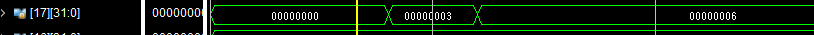
\includegraphics[scale=0.6]{add.png}
    \end{figure}
    \begin{figure}[H]
        \centering
        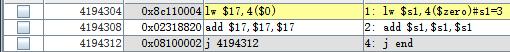
\includegraphics[scale=0.9]{addon.png}
        \end{figure}
一般load-store处理效果如下:
\begin{figure}[H]
    \centering
    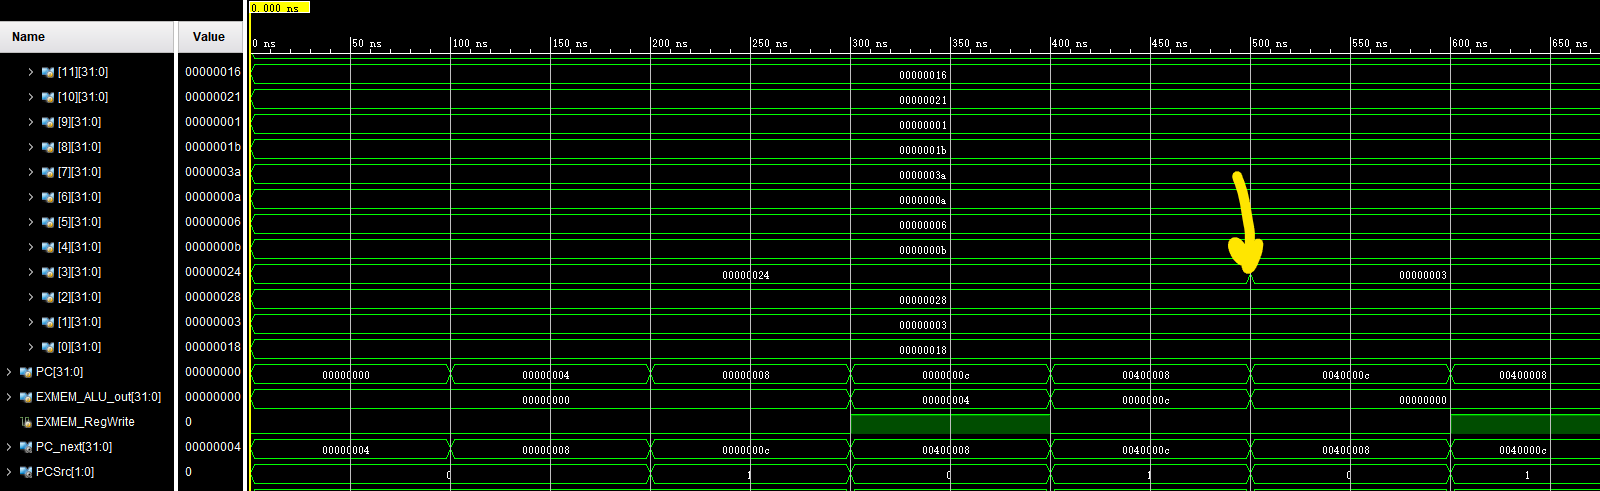
\includegraphics[scale=0.4]{lstore.png}
    \end{figure}
    \begin{figure}[H]
        \centering
        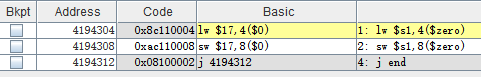
\includegraphics[scale=0.9]{fo.png}
        \end{figure}
特殊load-store处理效果如下:
\begin{figure}[H]
    \centering
    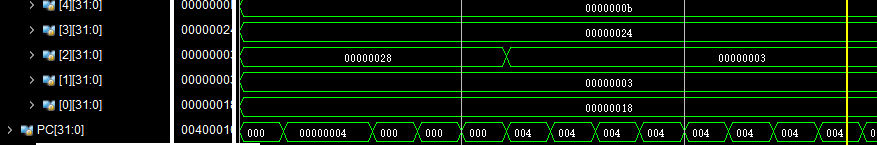
\includegraphics[scale=0.5]{specialls.png}
    \end{figure}
\begin{figure}[H]
    \centering
    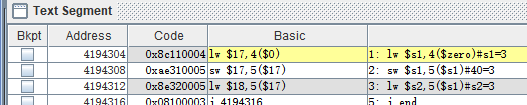
\includegraphics[scale=0.9]{hdl.png}
    \end{figure}

    另外,load后若紧跟Branch指令且发生冒险,则需要stall两个周期,
    暂不作处理,通过代码添加3个nop指令(0x00000000)解决。

    至此,数据冒险基本解决。
\subsection{控制冒险}
由于提前到ID阶段判断,分支指令、跳跃指令的下一条指令必然为nop。据此设定
修改即可。

利用流水线处理器排序结果如下:
\begin{figure}[H]
    \centering
    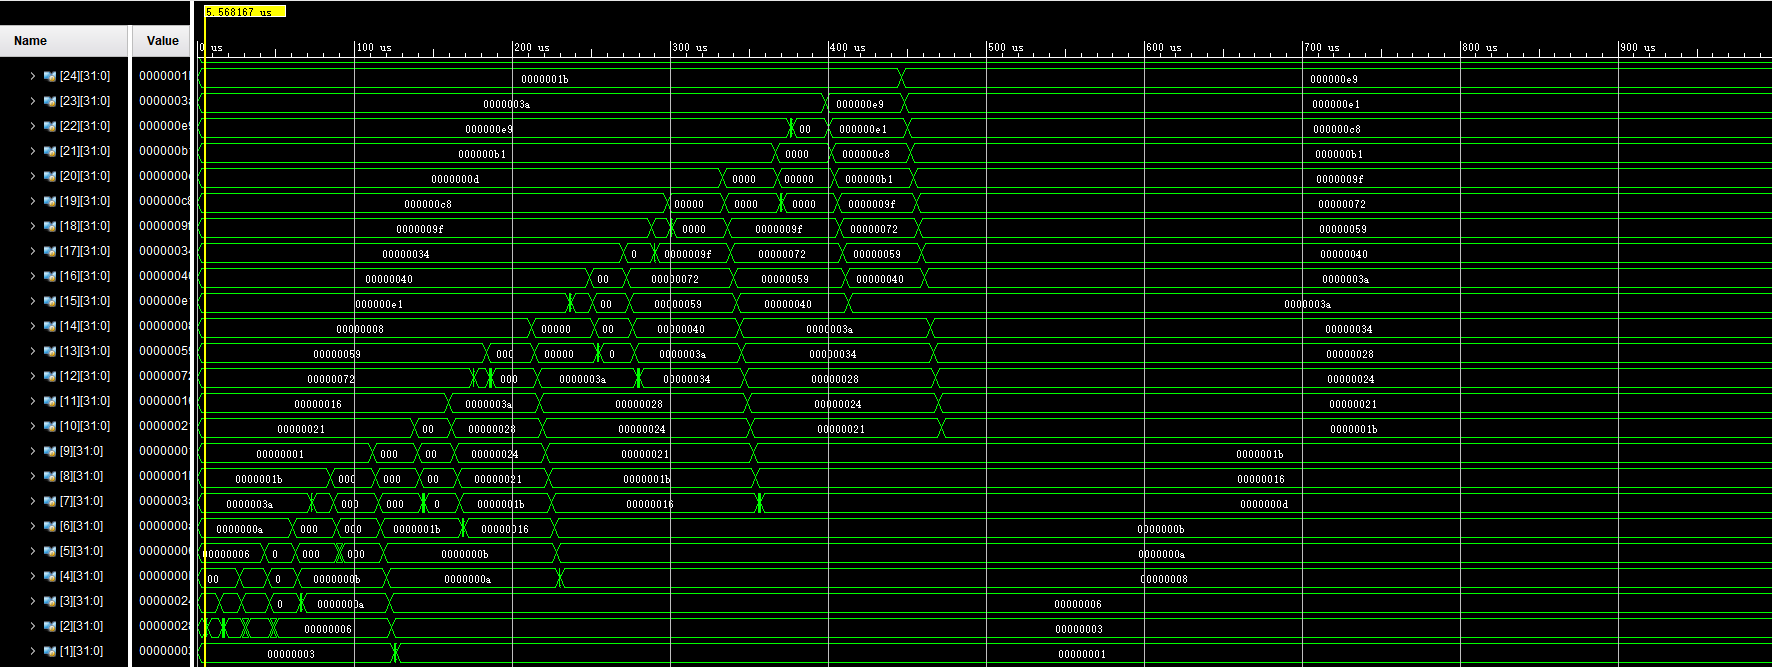
\includegraphics[scale=0.3]{mult.png}
    \end{figure}

\section{外设配置}

\end{document}










